\documentclass[crop,tikz]{standalone}
\usetikzlibrary{backgrounds}
\colorlet{blue}{cyan}
\tikzset{
  inverted/.style = {
    color=white,
    background rectangle/.style={fill},
    show background rectangle
  }
}

\usepackage{pgfplots}
\pgfplotsset{compat=1.16}

\tikzset{>=latex}

\pgfplotsset{
  inverted/.style = {
    every axis legend/.append style={
      draw=white,
      fill=black,
      text=white
    }
  },
  every non boxed x axis/.append style={
    axis line style={-latex}
  },
  every non boxed y axis/.append style={
    axis line style={-latex}
  }
}

\colorlet{green}{green}

\newcommand{\avg}[1]{\langle #1\rangle}
\newcommand{\std}[1]{s_{#1}}

\begin{document}
  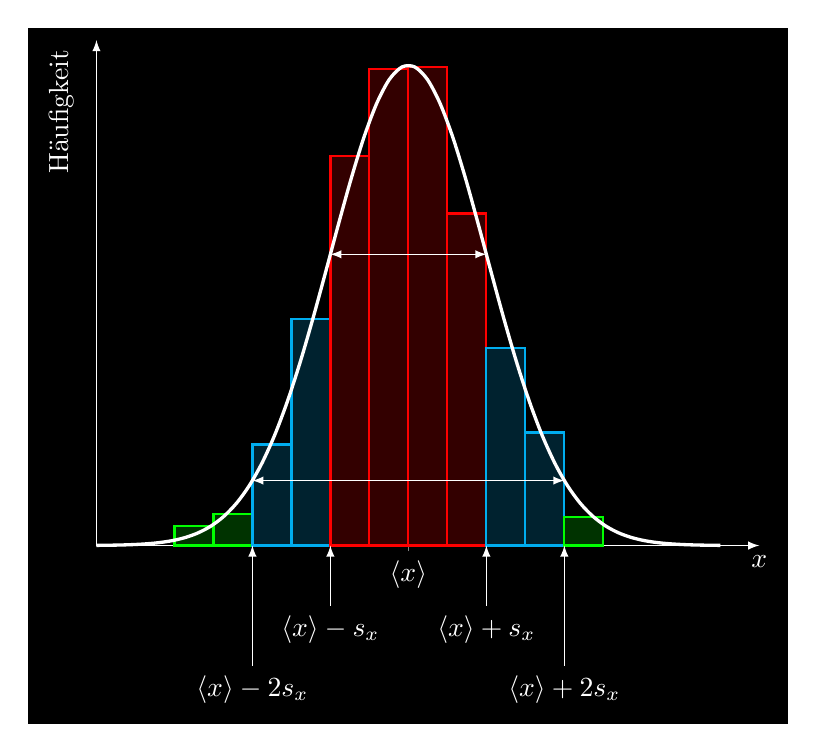
\begin{tikzpicture}[inverted,
    declare function = {
      gauss(\x,\sig,\mue) = 1/(sqrt(2*pi*\sig*\sig))*exp(-pow(\x-\mue,2)/(2*\sig*\sig)); 
    },
    ]
    \pgfmathsetmacro{\sig}{1}
    \pgfmathsetmacro{\mue}{4}
    \begin{axis}[inverted,
      width={10cm},
      height={8cm},
      axis y line=middle,
      axis x line=middle,
      xlabel={$x$},
      ylabel={Häufigkeit},
      x label style={below},
      y label style={at={(axis description cs:-0.02,1)},rotate=90,anchor=south east},
      ytick distance=0.1,
      domain=0:8,
      xmin=0, xmax=8.5,
      ymin=0, ymax=0.42,
      samples=50,
      xtick={\mue},
      xticklabels={$\avg{x}$},
      ymajorticks=false,
      clip=false,
      ]
      % BinCounts[RandomVariate[NormalDistribution[0,1], 1000], {-5,5,1/2}] // 1000
      \addplot[green, thick, ybar interval, mark=no, style={fill=green, fill opacity=0.2}] plot coordinates {
        (-3.  + 4, 2*0.008)
        (-2.5 + 4, 2*0.013)
        (-2.  + 4, 2*0.042)
      };
      \addplot[blue, thick, ybar interval, mark=no, style={fill=blue, fill opacity=0.2}] plot coordinates {
        (-2.  + 4, 2*0.042)
        (-1.5 + 4, 2*0.094)
        (-1.  + 4, 2*0.162)
      };
      \addplot[red, thick, ybar interval, mark=no, style={fill=red, fill opacity=0.2}] plot coordinates {
        (-1.  + 4, 2*0.162)
        (-0.5 + 4, 2*0.198)
        (0.   + 4, 2*0.199)
        (0.5  + 4, 2*0.138)
        (1.   + 4, 2*0.082)
      };
      \addplot[blue, thick, ybar interval, mark=no, style={fill=blue, fill opacity=0.2}] plot coordinates {
        (1.   + 4, 2*0.082)
        (1.5  + 4, 2*0.047)
        (2.   + 4, 2*0.012)
      };
      \addplot[green, thick, ybar interval, mark=no, style={fill=green, fill opacity=0.2}] plot coordinates {
        (2.   + 4, 2*0.012)
        (2.5  + 4, 2*0.005)
      };
      \addplot[very thick,smooth] { gauss(x,\sig,\mue) };
      \draw[<->] (axis cs: {\mue-\sig},{gauss(\mue-\sig,\sig,\mue)})     -- (axis cs: {\mue+\sig},{gauss(\mue+\sig,\sig,\mue)});
      \draw[<->] (axis cs: {\mue-2*\sig},{gauss(\mue-2*\sig,\sig,\mue)}) -- (axis cs: {\mue+2*\sig},{gauss(\mue+2*\sig,\sig,\mue)});
      \draw[->] (axis cs: {\mue-\sig}  ,-0.05) node[below] {$\avg{x}-\std{x}$}  -- (axis cs: {\mue-\sig}  ,0);
      \draw[->] (axis cs: {\mue+\sig}  ,-0.05) node[below] {$\avg{x}+\std{x}$}  -- (axis cs: {\mue+\sig}  ,0);
      \draw[->] (axis cs: {\mue-2*\sig},-0.10) node[below] {$\avg{x}-2\std{x}$} -- (axis cs: {\mue-2*\sig},0);
      \draw[->] (axis cs: {\mue+2*\sig},-0.10) node[below] {$\avg{x}+2\std{x}$} -- (axis cs: {\mue+2*\sig},0);
    \end{axis}
  \end{tikzpicture}
\end{document}
